\documentclass[11pt]{article}
\usepackage[utf8]{inputenc}
\usepackage[T1]{fontenc}
\usepackage{amsmath,amssymb,amsthm}
\usepackage{geometry}
\usepackage{booktabs}
\usepackage{graphicx}
\geometry{margin=2.5cm}

\begin{document}

\section{Expérience 1 : récupération de conjonctions aléatoires}

\subsection{Principe}

Cette expérience reproduit le protocole de convergence de PCL (Belaid
et al., AAAI-25) : on tire une conjonction cible aléatoire, on entraîne
une seule clause dessus, et on vérifie si la clause apprise correspond
\emph{exactement} à la cible. L'objectif est de comparer directement
notre règle à quatre paramètres $(a,b,c,d)$ à la règle à un paramètre
$p$ de PCL, sur le terrain même de leur article.

\subsection{Protocole}

Pour chaque valeur de $n$ (nombre de features) :

\begin{enumerate}
\item \textbf{Génération de la cible.} On tire une cible aléatoire
$\text{target}\in\{0,1,2\}^n$ (0 : le littéral $\neg x_i$ doit être
présent, 1 : le littéral $x_i$ doit être présent, 2 : la feature $i$
est inutile), avec une garde contre le cas où toutes les features
seraient inutiles.

\item \textbf{Construction de la table de vérité complète.} On génère
les $2^n$ entrées possibles $x\in\{0,1\}^n$ et leur label $y$ associé
(sans bruit), déterminé par la cible.

\item \textbf{Entraînement.} On entraîne une seule clause sur cette
table, pendant $100$ epochs (un epoch = un passage complet sur les
$2^n$ lignes, dans le même ordre à chaque fois) :
\begin{itemize}
\item avec le code officiel non modifié de PCL (\texttt{PCL\_convergence\_all.py},
dépôt \texttt{cair/dpcl-classifier}) ;
\item avec notre règle à quatre paramètres $(a,b,c,d)$ (Définition~1).
\end{itemize}

\item \textbf{Critère de succès.} On extrait la clause apprise
(l'ensemble des littéraux inclus) et on la compare à la cible. Un essai
est un succès si et seulement si les deux ensembles de littéraux
coïncident exactement (récupération exacte, pas juste bonne précision).

\item \textbf{Répétition.} Cette procédure est répétée $100$ fois (100
cibles aléatoires différentes), ce qui donne un score sur $100$. Toute
la procédure est elle-même répétée $10$ fois (comme dans le protocole
de PCL), et le chiffre rapporté est la moyenne de ces $10$ scores.
\end{enumerate}

\subsection{Paramètres}

\begin{center}
\begin{tabular}{ll}
\toprule
Paramètre & Valeur \\
\midrule
Nombre de features $n$ & $1,2,\ldots,12$ \\
Nombre d'états par automate (states) & $N=10\,000$ \\
Nombre d'epochs & $100$ \\
Probabilité d'inclusion PCL ($p$) & $0.95$ (réglage ``PCL-a'', table complète) \\
Paramètres de notre règle $(a,b,c,d)$ & $a=1.0,\ b=0.3,\ c=1.0,\ d=0.1$ \\
& (respecte $a,b,c,d\in(0,1]$ et l'Hypothèse~1 : $a\le c$, $d\le b$) \\
Nombre de cibles aléatoires par run & $100$ \\
Nombre de runs (répétitions) & $10$ \\
Nombre total d'essais par valeur de $n$ & $1\,000$ \\
\bottomrule
\end{tabular}
\end{center}

\subsection{Résultats}

\begin{center}
\begin{tabular}{cccc}
\toprule
$n$ & PCL (publié, Tableau 7) & PCL (notre reproduction) & Notre règle \\
\midrule
1  & --    & 100.0 & 100.0 \\
2  & --    & 99.5  & 100.0 \\
3  & --    & 96.9  & 100.0 \\
4  & 95.1  & 94.4  & 100.0 \\
5  & 91.2  & 91.4  & 100.0 \\
6  & 86.1  & 85.3  & 99.9  \\
7  & 79.4  & 77.9  & 100.0 \\
8  & 69.3  & 68.9  & 100.0 \\
9  & 57.1  & 56.6  & 100.0 \\
10 & 49.8  & 51.4  & 100.0 \\
11 & 42.3  & 43.6  & 100.0 \\
12 & 34.2  & 35.4  & 100.0 \\
\bottomrule
\end{tabular}
\end{center}

Les valeurs publiées de PCL-a (colonne 2) proviennent du Tableau~7 de
Belaid et al. (AAAI-25) ; ce papier ne teste pas $n<4$. Notre
reproduction (colonne 3, code officiel non modifié, mêmes paramètres
$p=0.95$) retombe systématiquement à moins de $1.5$ point de leurs
chiffres publiés, ce qui valide la fidélité de notre protocole
expérimental.

\subsection{Interprétation}

PCL se dégrade nettement et progressivement à mesure que $n$
augmente (de $100\%$ à $n=1$ jusqu'à $\sim35\%$ à $n=12$), un
comportement attendu vu que $0.5<p<1$ n'assure la convergence que sous
la loi uniforme, sans garantie sur la vitesse de convergence en
fonction de $n$. Notre règle, elle, reste à $100\%$ sur toute la
plage testée (à l'exception d'un seul essai malchanceux sur les $1\,000$
à $n=6$, donnant $99.9\%$ au lieu de $100\%$) : à budget d'epochs
identique, elle converge nettement plus vite que PCL quand $n$
grandit.

\section{Expérience 2 : robustesse au bruit (Théorème 5)}

\subsection{Principe}

Le Théorème 5 affirme que, sous l'Hypothèse~1, si le niveau de bruit
$\eta$ (probabilité qu'un label soit inversé) reste strictement en
dessous d'un seuil $\eta_{\max}=\mu/M$ propre à chaque cible, alors la
règle identifie toujours exactement la cible malgré le bruit. Ici $\mu$
est la marge minimale sur les $2n$ dérives (calculée à partir des
données propres, sans bruit) et $M=\max(a+b,\,c+d)$.

Contrairement à l'Expérience~1, il ne s'agit pas de comparer à PCL :
PCL n'a pas d'équivalent prouvé à ce théorème, la comparaison n'aurait
pas de sens. L'objectif est de vérifier directement, empiriquement, que
ce seuil $\eta_{\max}$ est réel.

\subsection{Protocole}

Pour rendre la comparaison indépendante de $n$ (le seuil $\eta_{\max}$
varie fortement avec $n$), on exprime le bruit testé par le rapport
$r=\eta/\eta_{\max}$ plutôt que par $\eta$ directement : $r<1$ correspond
à la zone garantie par le théorème, $r>1$ est hors garantie (simple
stress test empirique, sans promesse théorique).

Pour chaque valeur de $r$ testée :
\begin{enumerate}
\item On tire une cible aléatoire et sa table de vérité complète (comme
à l'Expérience~1), pour une valeur de $n$ tirée parmi $\{4,6,8,10,12\}$.
\item On calcule $\mu$ sur les données propres, puis
$\eta_{\max}=\mu/M$ et $\eta = r\times\eta_{\max}$ (plafonné à $0.5$,
au-delà duquel le bruit devient dégénéré).
\item On construit une table d'entraînement répétée $100$ fois (une par
epoch), en inversant chaque label indépendamment avec probabilité
$\eta$ \emph{à chaque répétition} (bruit frais à chaque epoch, pas figé
une fois pour toutes).
\item On entraîne notre règle sur cette table bruitée et on vérifie si
la clause apprise correspond exactement à la cible propre (non
bruitée).
\end{enumerate}
Cette procédure est répétée $200$ fois par valeur de $r$ (avec $n$
mélangé entre les essais), et on rapporte le taux de succès.

\subsection{Paramètres}

\begin{center}
\begin{tabular}{ll}
\toprule
Paramètre & Valeur \\
\midrule
Nombre de features $n$ & tiré parmi $\{4,6,8,10,12\}$ \\
Nombre d'états par automate (states) & $N=10\,000$ \\
Nombre d'epochs & $100$ \\
Paramètres de notre règle $(a,b,c,d)$ & $a=1.0,\ b=0.3,\ c=1.0,\ d=0.1$ \\
Valeurs de $r=\eta/\eta_{\max}$ testées & $0.2,\ 0.5,\ 1,\ 2,\ 5,\ 10,\ 20,\ 50,\ 100,\ 200,\ 500$ \\
Nombre d'essais par valeur de $r$ & $200$ \\
\bottomrule
\end{tabular}
\end{center}

\subsection{Résultats}

\begin{center}
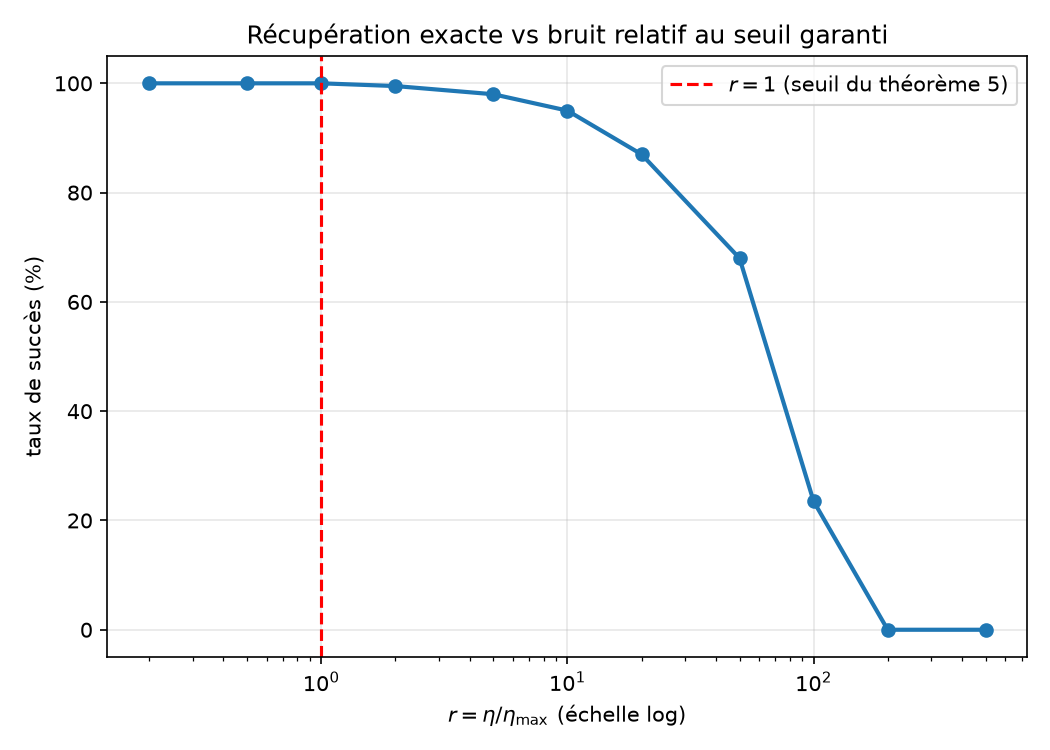
\includegraphics[width=0.85\textwidth]{figures/succes_vs_r_theoreme5.png}
\end{center}

\begin{center}
\begin{tabular}{ccccccccccc}
\toprule
$r$ & 0.2 & 0.5 & 1 & 2 & 5 & 10 & 20 & 50 & 100 & 200 & 500 \\
\midrule
succès (\%) & 100.0 & 100.0 & 100.0 & 100.0 & 98.0 & 95.0 & 87.0 & 67.5 & 23.5 & 0.0 & 0.0 \\
\bottomrule
\end{tabular}
\end{center}

\subsection{Interprétation}

Le taux de succès reste exactement à $100\%$ jusqu'à $r=2$, soit bien
au-delà du seuil garanti $r=1$ : pour ce choix de paramètres
($a+b=1.3\ne c+d=1.1$), la borne du Théorème~5 est prudente (non
serrée) -- le Théorème~5(2) précise que la borne n'est exactement
optimale que lorsque $a+b=c+d$. La dégradation commence ensuite
progressivement à partir de $r\approx5$, pour s'effondrer complètement
entre $r=100$ et $r=200$. Ce résultat confirme empiriquement le seuil
du Théorème~5 : rien n'indique de rupture avant $r=1$, et la règle
tolère en pratique un bruit nettement supérieur à ce que la théorie
garantit formellement pour ce jeu de paramètres.

\end{document}
